\documentclass[xcolor=dvipsnames]{beamer}
%\usetheme[progressbar=frametitle]{metropolis}
\usecolortheme{seahorse}

\definecolor{gray}{HTML}{151515}
\definecolor{orange}{HTML}{d28445}

\setbeamercolor{normal text}{fg=gray}
\setbeamercolor{progress bar}{fg=orange}

% balíčky

\usepackage[utf8]{inputenc}
\usepackage[czech]{babel}
\usepackage{graphicx, tabularx}
\usepackage{amsmath, amssymb, amsthm}
\newcommand{\abs}[1]{\lvert #1 \,\rvert} %}}}
\usefonttheme[onlymath]{serif}	
\usepackage{dashrule}

%gets rid of bottom navigation bars
\setbeamertemplate{footline}[frame number]{}

%gets rid of bottom navigation symbols
\setbeamertemplate{navigation symbols}{}

%gets rid of footer
%will override 'frame number' instruction above
%comment out to revert to previous/default definitions
\setbeamertemplate{footline}{} 

\usepackage{asymptote}
\usepackage{epstopdf}
\usepackage{xcolor}

\usepackage[backend=biber, url=true, sorting=none]{biblatex}
\renewcommand*{\bibfont}{\footnotesize}
\addbibresource{../soc.bib}
\usepackage{url}

\title{Mechanika rodin planetek \\ s aplikací na rodinu Eunomia}
\author{Adam Křivka \\ \and doc. Mgr. Miroslav Brož, Ph.\,D.}
\institute{Cyrilometodějské gymnázium a střední odborná škola pedagogická Brno,\\ Lerchova 63, 602 00 Brno}

\begin{document}

\begin{frame}
\titlepage
\end{frame}

{
\setbeamerfont{section in toc}{shape=\bfseries}
\setbeamercolor{section in toc}{fg=white}

\section{Úvod}
\setbeamertemplate{frametitle}{}
% \usebackgroundtemplate{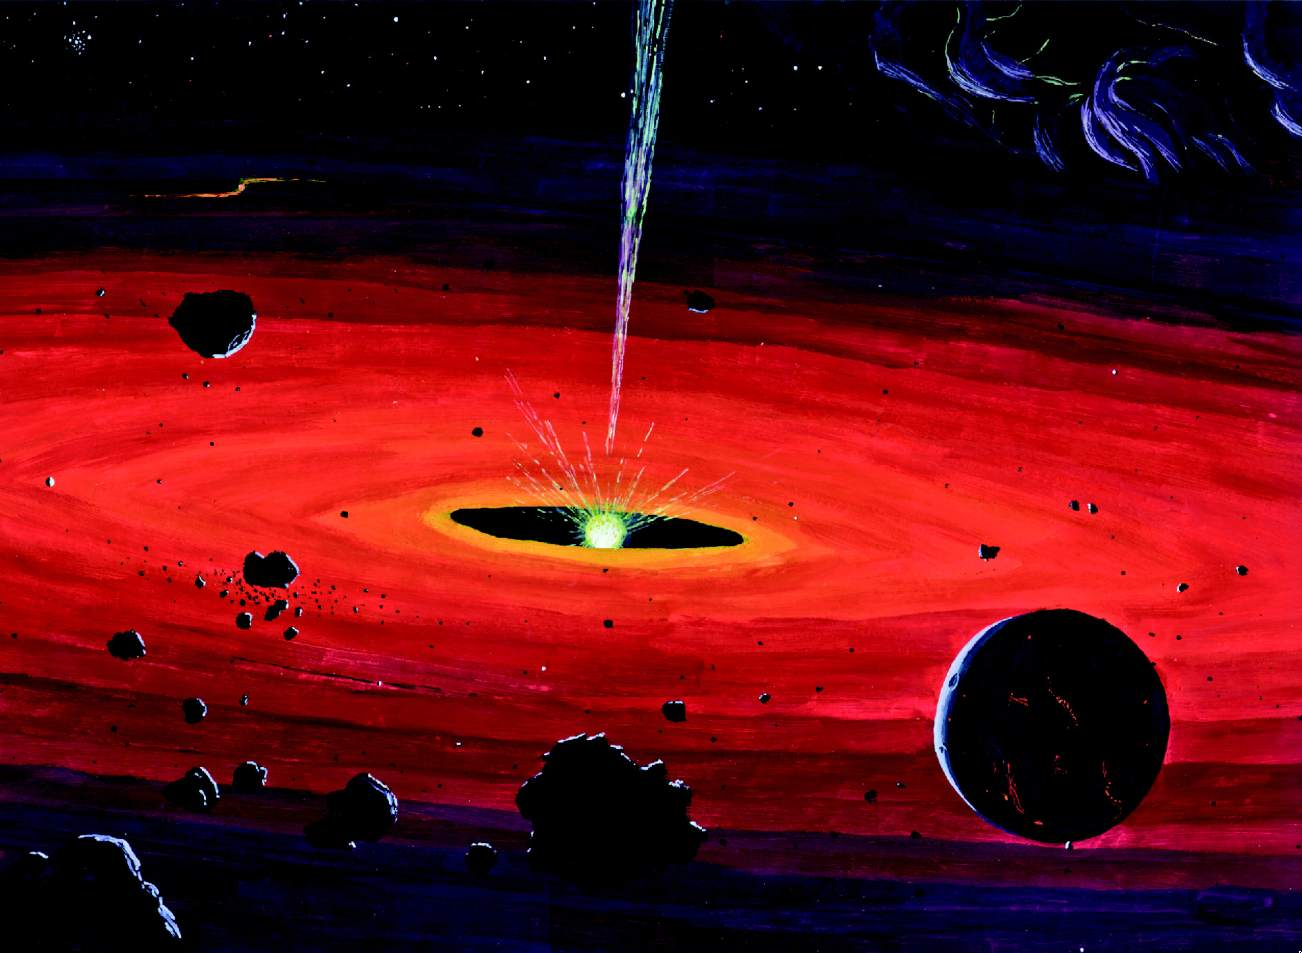
\includegraphics[width=\paperwidth]{../obr/fmt.jpg}}%
\usebackgroundtemplate{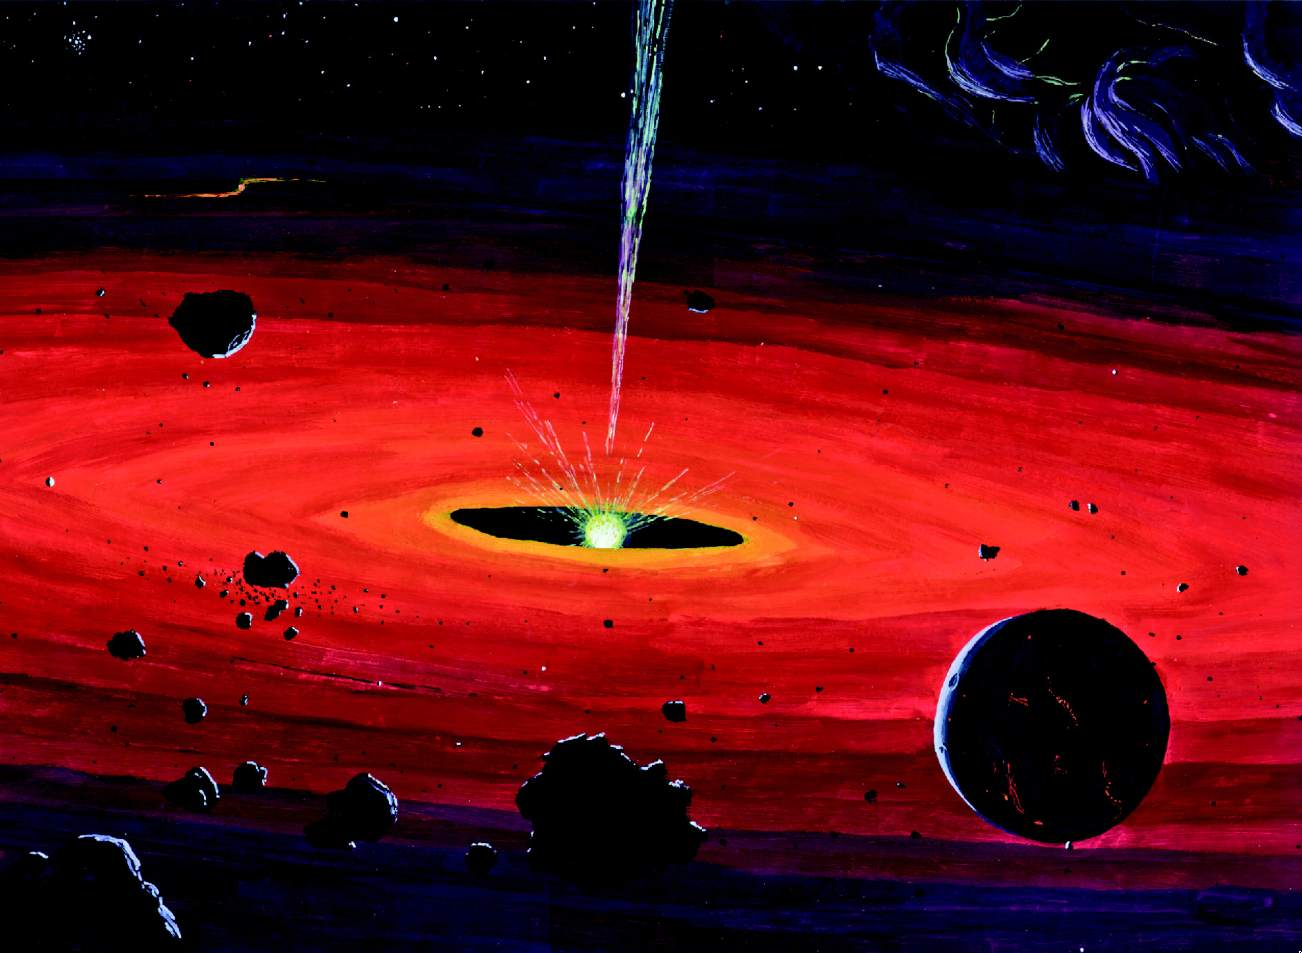
\includegraphics[height=\paperheight]{../obr/fmt.jpg}}%
\begin{frame}{Úvod}
\textcolor{white}{\tableofcontents}
\end{frame}
}

\section{Nebeská mechanika}
\begin{frame}{\secname}{Problém $N$ těles}
\begin{figure}
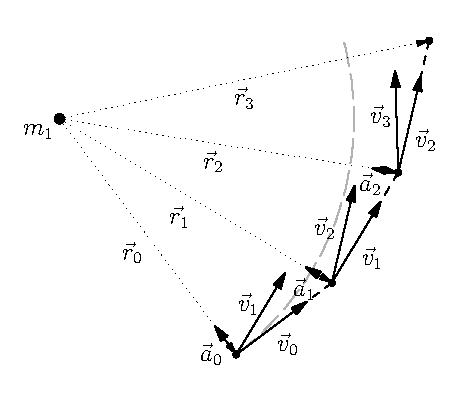
\includegraphics[width=0.49\textwidth]{../asy/asteroidy-3.pdf}
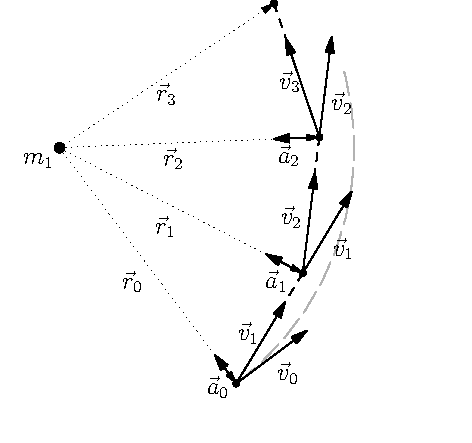
\includegraphics[width=0.49\textwidth]{../asy/asteroidy-4.pdf}
\vspace{-1cm}
\caption{\footnotesize{Ilustrace dopředné (vlevo) a zpětné (vpravo) Eulerovy metody pro výpočet problému dvou těles.}}
\end{figure}
\vspace{-0.5cm}
\begin{align*}
m_i\vec{a}_i &= -\sum_{\substack{j=1 \\ j\neq i}}^N \frac{Gm_im_j}{\abs{\vec{r}_i-\vec{r}_j}^3}(\vec{r_i}-\vec{r_j})\,, \qquad{\rm pro}\ i\in\{1,\,2,\,\dots,\,N\} \label{eq:nbody2}
\end{align*}
\end{frame}

\begin{frame}{\secname}{Elementy dráhy}
\begin{columns}
\begin{column}{0.5\textwidth}
\begin{itemize}
\item Velká poloosa $a\,[{\rm AU}]$  
\item Excentricita $e$
\item Sklon $i\,[ ^\circ]$
\item Argument pericentra $\omega\,[ ^\circ]$
\item Délka vzestupného uzlu $\Omega\,[ ^\circ]$
\item Střední anomálie $M \,[ ^\circ]$
\end{itemize}
\end{column}
\begin{column}{0.5\textwidth}
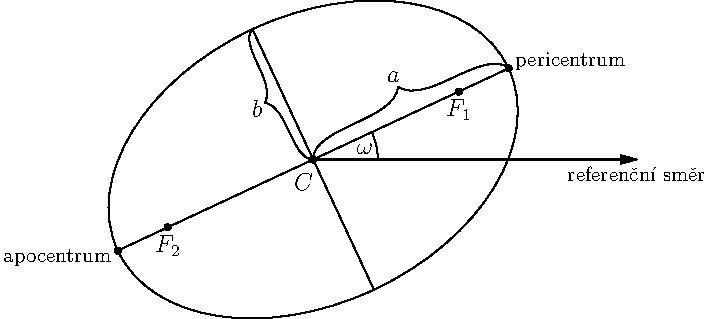
\includegraphics[width=1.1\textwidth]{../asy/asteroidy-1.pdf}
\
\begin{align*}
	e=\sqrt{1-\frac{b^2}{a^2}}
\end{align*}
\end{column}
\end{columns}
\end{frame}

\section{Planetky ve sluneční soustavě}
\begin{frame}{\secname}{Tvar a vznik}
\begin{figure}
\centering
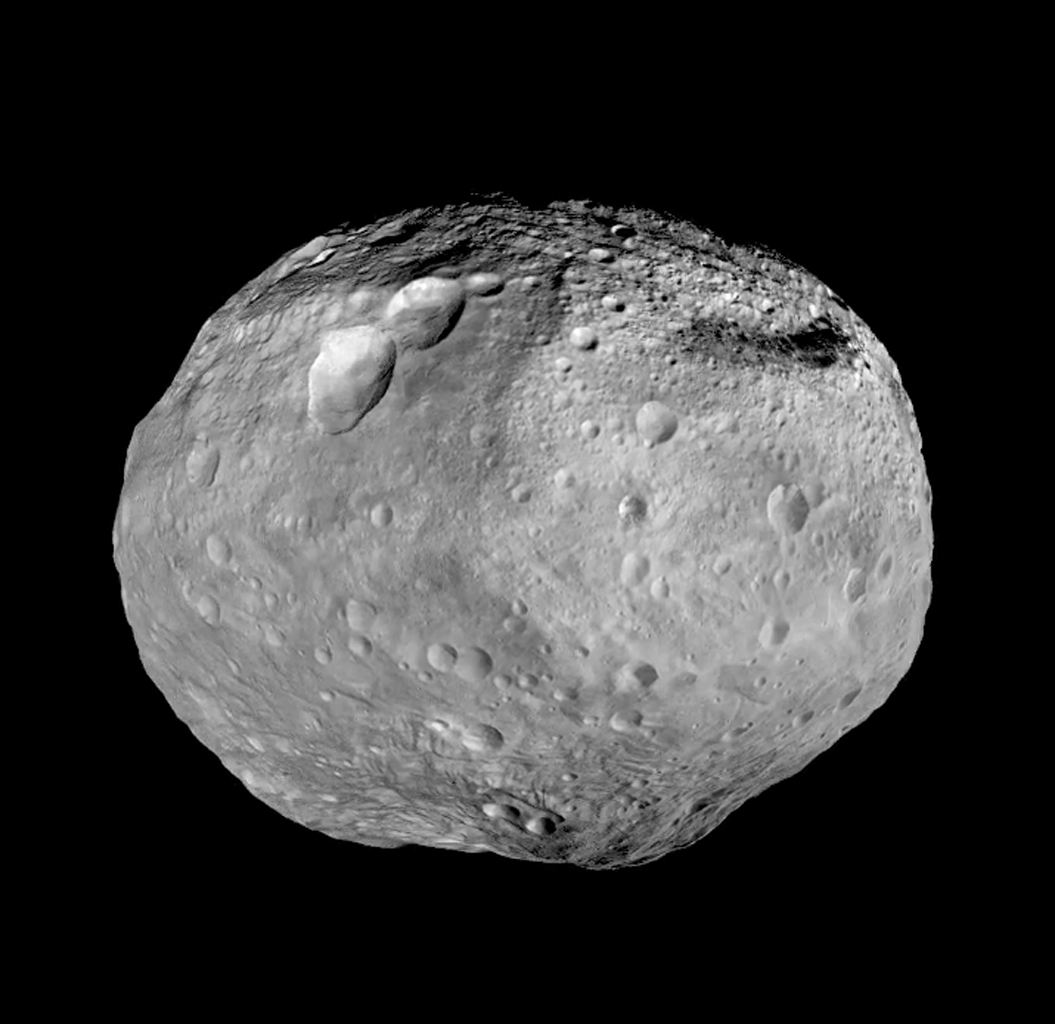
\includegraphics[height=0.7\textheight,width=\textwidth,keepaspectratio]{../obr/vesta.jpg}
\caption{\footnotesize{Planetka (4) Vesta. Fotografie byla pořízena americkou sondou \textit{Dawn}. Převzato z~\cite{jplvesta}.}}
\end{figure}
\end{frame}

\begin{frame}{\secname}{Rodiny planetek}
\begin{figure}
\centering
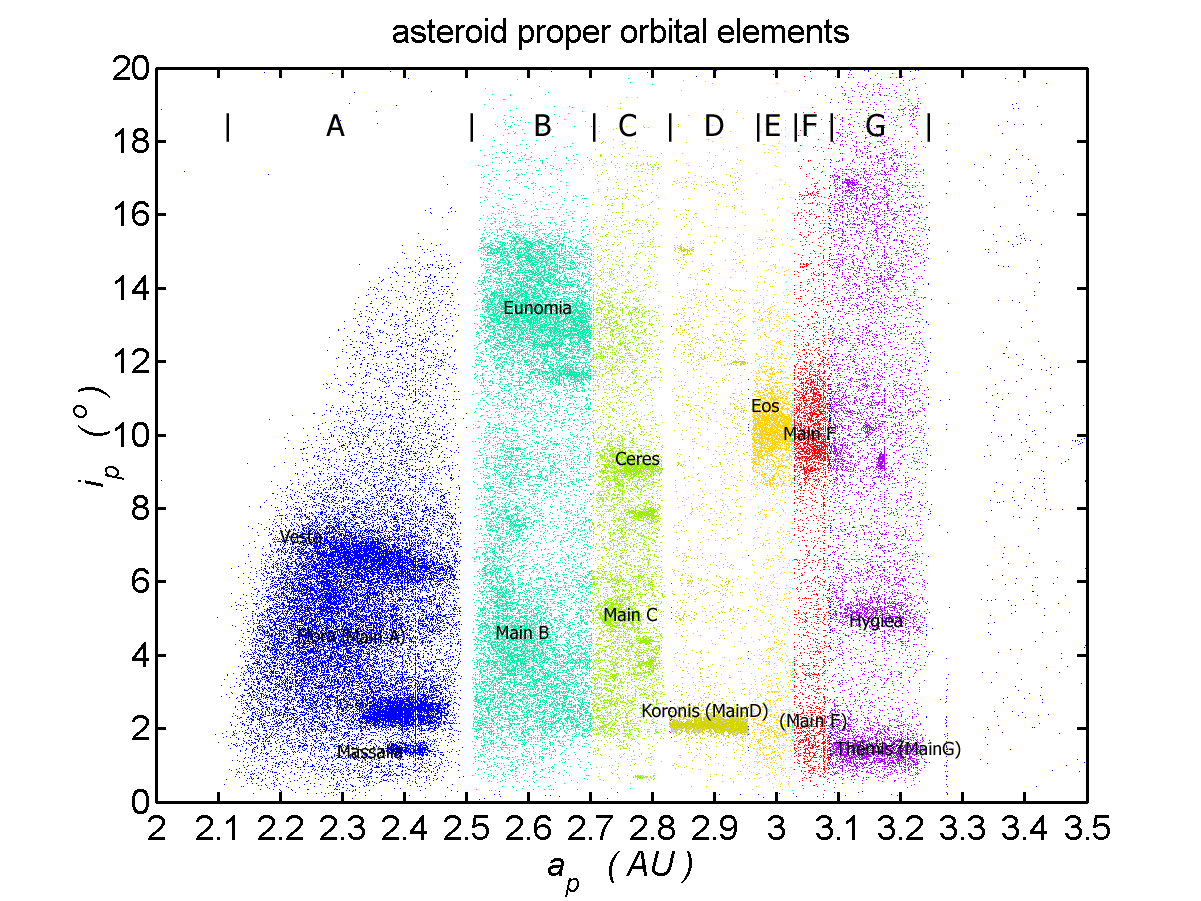
\includegraphics[height=0.7\textheight,width=\textwidth,keepaspectratio]{../obr/mainbelt.png}
\caption{\footnotesize{Planetky hlavního pásu podle vlastních elementů dráhy --- vlastní velké poloosy $a_{\rm p}$ a vlastního sklonu $i_{\rm p}$. Převzato z~\cite{wiki:belt}.}}
\end{figure}
\end{frame}

\section{Vlastnosti rodiny Eunomia}
\begin{frame}[t]{\secname}{Identifikace a rozdělení}
\vspace{-1cm}
\begin{figure}
\centering
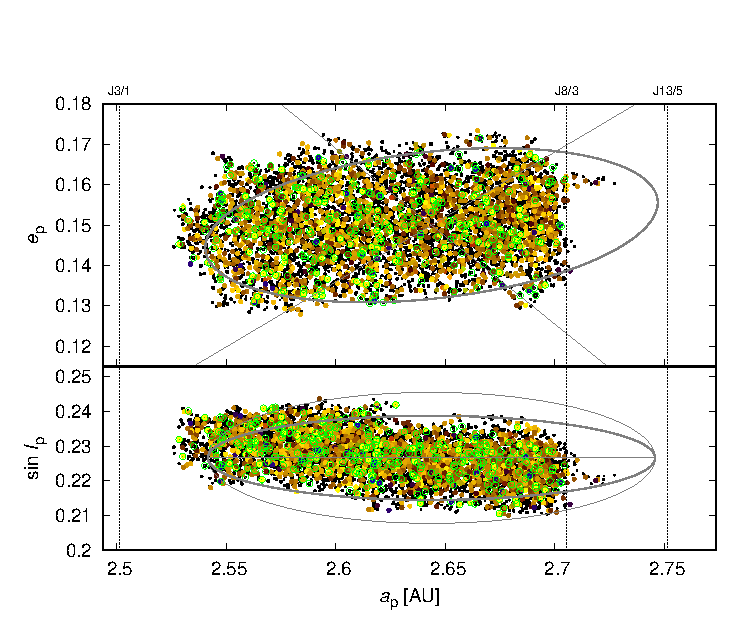
\includegraphics[width=0.8\textwidth]{../obr/ae_ai_wise}
\caption{\footnotesize{Pozorovaná rodina Eunomia v~rovině vlastní hlavní poloosy $a_{\rm p}$ a vlastní excentricity $e_{\rm p}$, identifikovaná \textit{hierarchickou shlukovací metodou}. Barevná škála odpovídá albedu $p_{\rm V}$ a $p_{\rm IR}$ z~katalogu WISE\@.}}
\end{figure}
\end{frame}

\begin{frame}[t]{\secname}{Barevné charakteristiky}
\begin{figure}
\centering
\includegraphics[width=0.7\textwidth]{../obr/pV_pIR}
\caption{\footnotesize{Albeda $p_{\rm V}$ a $p_{\rm IR}$ z~katalogu WISE. Pro vyřazení přimísených byly zvoleny hraniční hodnoty $0,05 \leq p_{\rm V} \leq 0,4$.}}
\end{figure}
\end{frame}

\begin{frame}[t]{\secname}{Jarkovského a YORP jev}
\begin{figure}
\centering
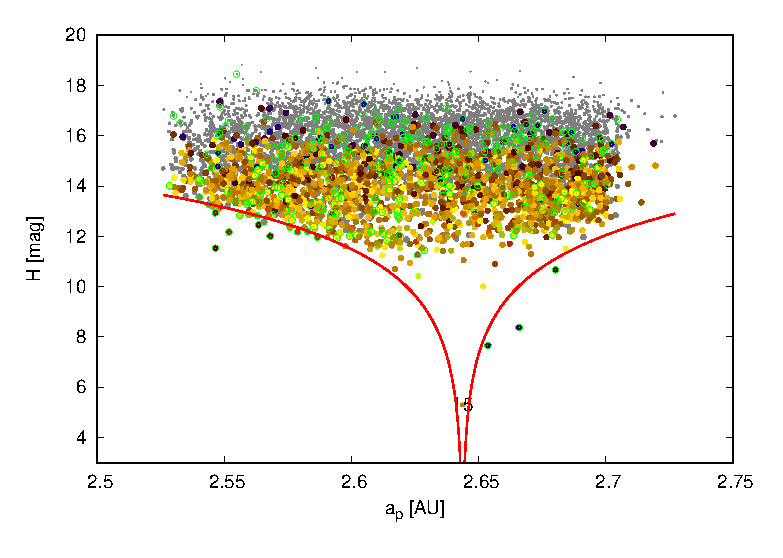
\includegraphics[width=0.7\textwidth]{../obr/aH_wise.eps}
\caption{\footnotesize{Rozdělení pozorované rodiny \textit{Eunomia} v~rovině vlastní hlavní poloosy $a_{\rm p}$ a absolutní hvězdné velikosti $H$. Lze pozorovat typický tvar \uv{V}, který je způsobem počátečním rychlostním polem a Jarkovského jevem.}}
\end{figure}
\end{frame}

\begin{frame}[t]{\secname}{Výsledky simulace}
\centering
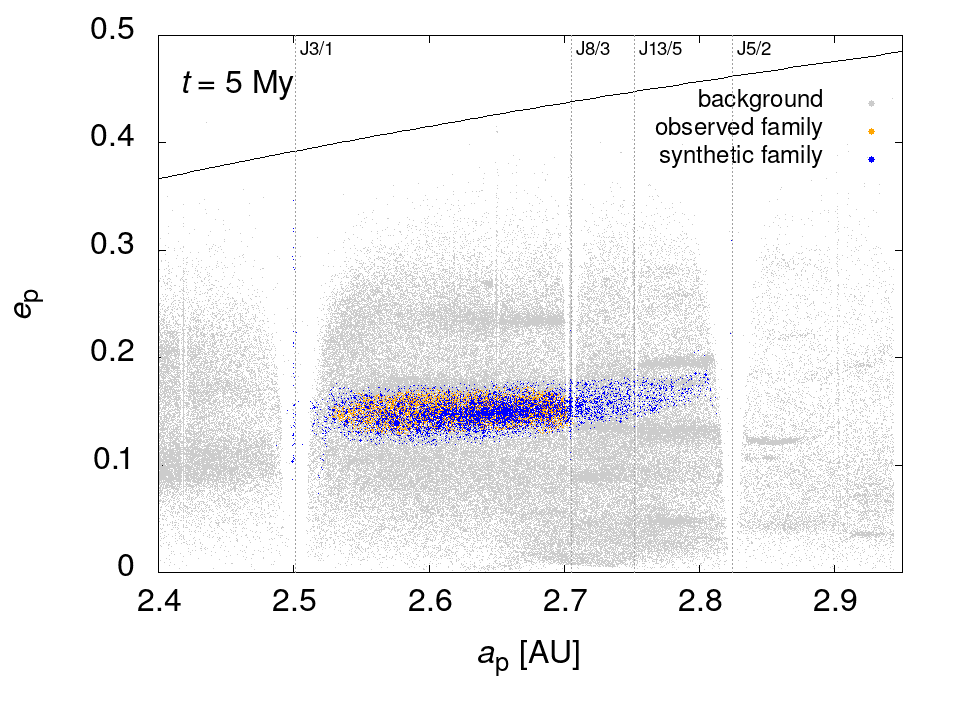
\includegraphics[width=0.8\paperwidth]{../obr/ae_5_trans.png}
\end{frame}

\begin{frame}[t]{\secname}{Analýza chí kvadrátu}
\centering
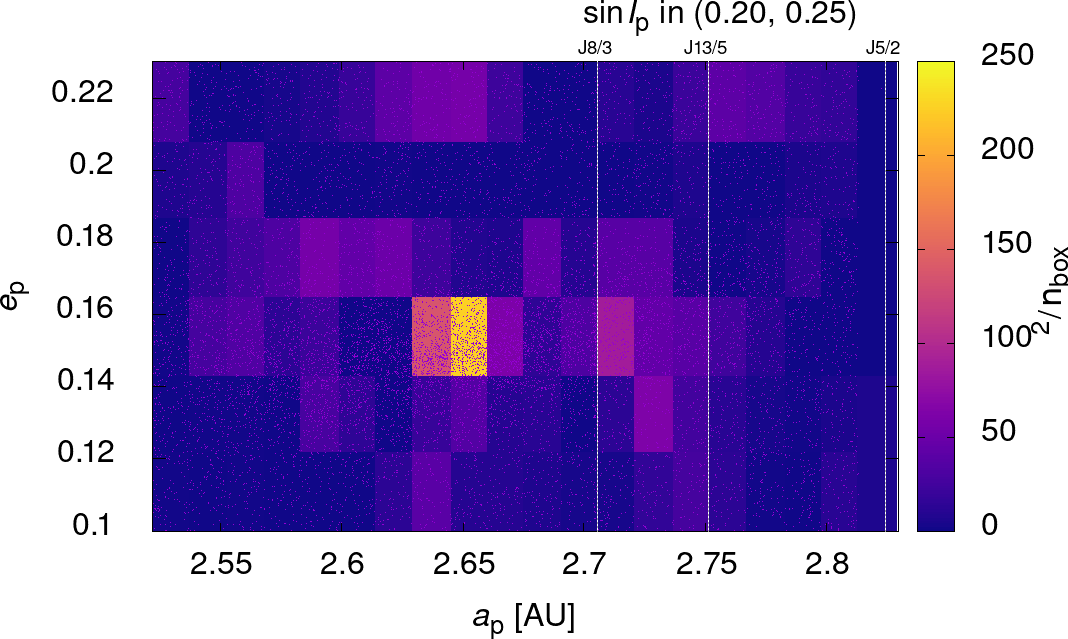
\includegraphics[width=0.41\paperwidth]{../obr/ae_chi_0006t.png}
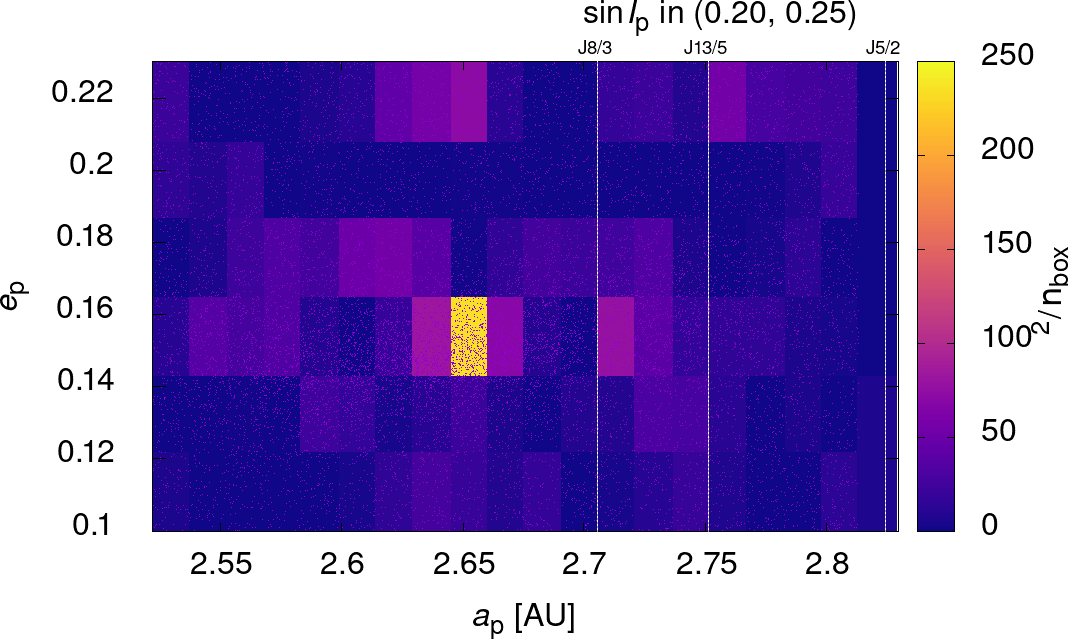
\includegraphics[width=0.41\paperwidth]{../obr/ae_chi_0106t.png}\\
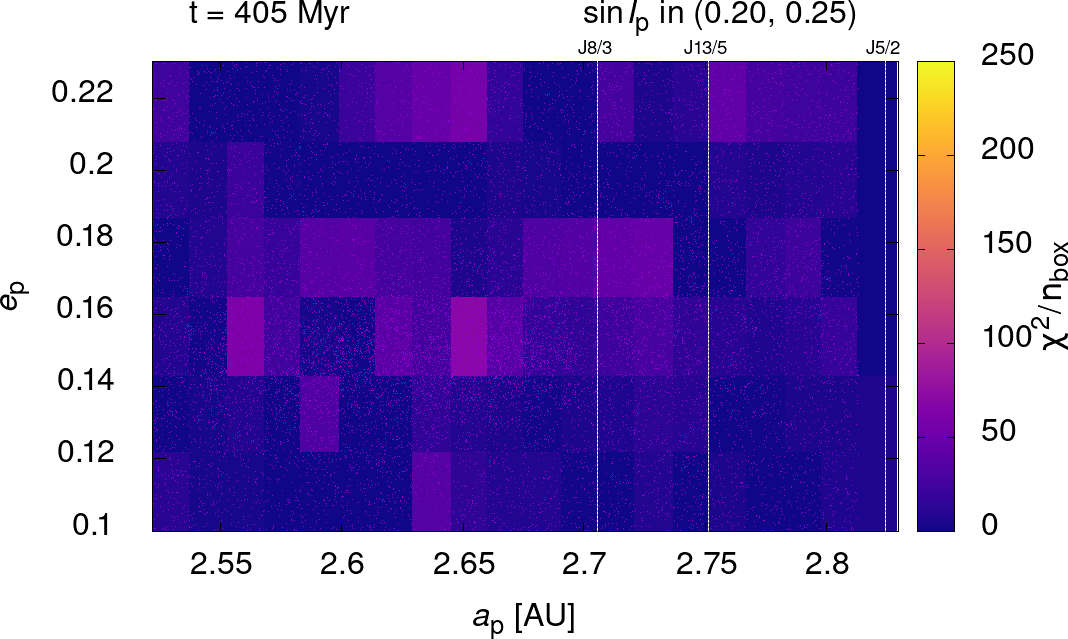
\includegraphics[width=0.41\paperwidth]{../obr/ae_chi_0406t.png}
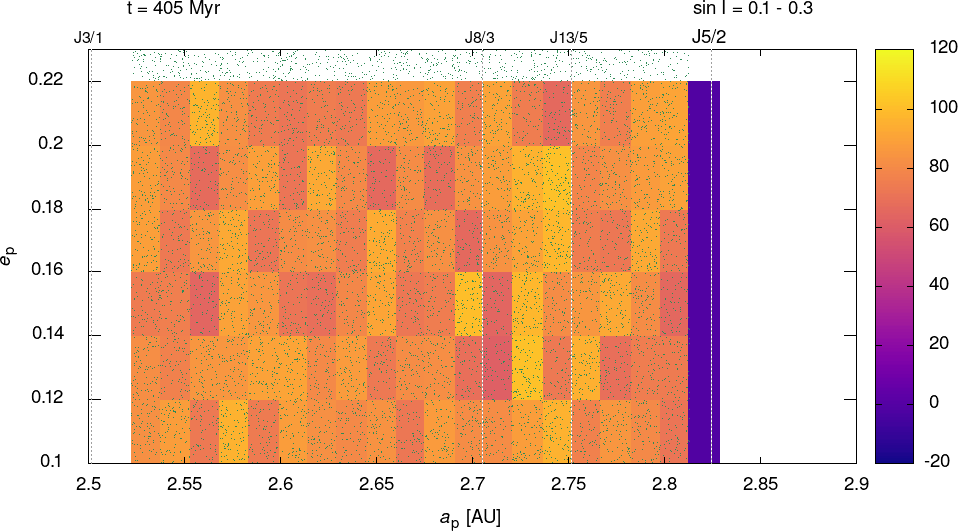
\includegraphics[width=0.41\paperwidth]{../obr/ae_chi_emptyt.png}
\end{frame}

\begin{frame}[t]{\secname}{Porovnání simulované a pozorované rodiny}
\newcolumntype{V}{>{\centering\arraybackslash} m{.4\linewidth} }
\begin{tabularx}{\textwidth}{c V}
\centering
Simulovaná: & \includegraphics[width=0.46\paperwidth]{../obr/ae_scl.png}\\
Pozorovaná: & \includegraphics[width=0.46\paperwidth]{../obr/ae_obs.png}
\end{tabularx}
\end{frame}

\begin{frame}[c]{\secname}{Vývoj chí kvadrátu}
\centering
\includegraphics[width=0.5\textwidth]{../obr/chi2.eps}
\end{frame}

\section{Závěr}
\begin{frame}[t]{\secname}{Reference a doporučená literatura}
	\printbibliography

{\color{blue}
	\hdashrule[0.5ex]{\textwidth}{0.7pt}{2mm}}

	\newrefsection{}
	\setbeamertemplate{bibliography item}[book]
	\nocite{fmt}
	\nocite{murray00}
	\nocite{brozphd}
	\printbibliography
\end{frame}
\begin{frame}
Děkuji za pozornost.
\end{frame}
\end{document}
